\chapter{Découvrons le LoPy}

\textit{Les programmes relatifs à cette section se trouvent dans le répertoire \texttt{plido-tp3} pour le serveur et \texttt{pycom} pour le LoPy.}

\section{Introduction}

Grâce aux émulateurs de capteurs décrits au chapitre précédent, vous avez pu appliquer les concepts essentiels de l'IoT sur votre ordinateur.

Cependant, si vous le pouvez, nous vous invitons à le faire sur de vrais objets connectés en utilisant des \Index{LoPy4} (plateforme de prototypage IoT) de la société \Index{Pycom} et des capteurs de température, humidité et pression \Index{BME280} (cf. figure~\vref{fig-lopy-bme280}). 

\begin{figure}[tbp]
\centerline{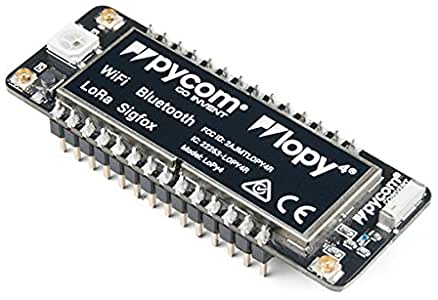
\includegraphics[width=.5\columnwidth]{Pictures/LoPy.jpg}  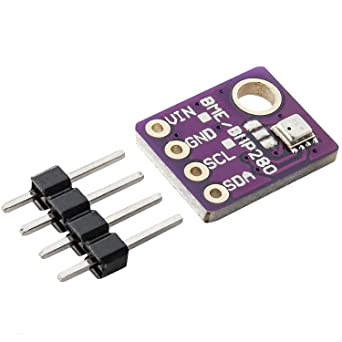
\includegraphics[width=.3\columnwidth]{Pictures/BME280.jpeg}}
\caption{LoPY4 et capteur BME280}
\label{fig-lopy-bme280}
\end{figure}

Un LoPY4 se programme en Python (ou plutôt \Index{MicroPython} qui est la version du langage pour systèmes embarqués) pour traiter les données. Dans un premier temps, nous allons utiliser le Wi-Fi pour communiquer avec votre ordinateur mais, par la suite, nous mettrons en place une communication via \Index{LoraWAN} ou \Index{Sigfox} qui peut vous demander plus de configuration mais vous permettra de mieux comprendre ces protocoles.

     \vspace{1em}


Même si vous n’avez pas de LoPy4, vous pouvez parcourir cette section pour voir les contraintes supplémentaires liées aux objets connectés.

\section{Installation d'Atom}

\Index{Atom} est un éditeur de texte performant, spécifiquement conçu pour le codage en différents langages. 
Atom va nous aider à programmer en Python et va également gérer la communication avec notre LoPy via le port \Index{USB} (grâce au plugin \Index{Pymakr}). Atom fonctionne à peu près de la même manière sur \Index{Mac OS}, \Index{Windows} et \Index{Linux}, mais en s’adaptant aux particularités du système d’exploitation (place dans les menus, nom des liens séries...). Donc, il se peut que vous ayez quelques différences entre ce que vous avez dans cet ouvrage et l’écran de votre ordinateur. Les menus et sites Web indiqués peuvent également changer au cours du temps même si nous nous efforçons de faire des mises à jour régulières du cours.


     \vspace{1em}

Pour commencer à programmer avec votre LoPy, vous devez installer sur votre ordinateur le logiciel Atom (voir sur \url{http://atom.io}). Vous pouvez télécharger le package correspondant à votre système d'exploitation (cf. figure suivante).

\begin{figure}[tbp]
\centerline{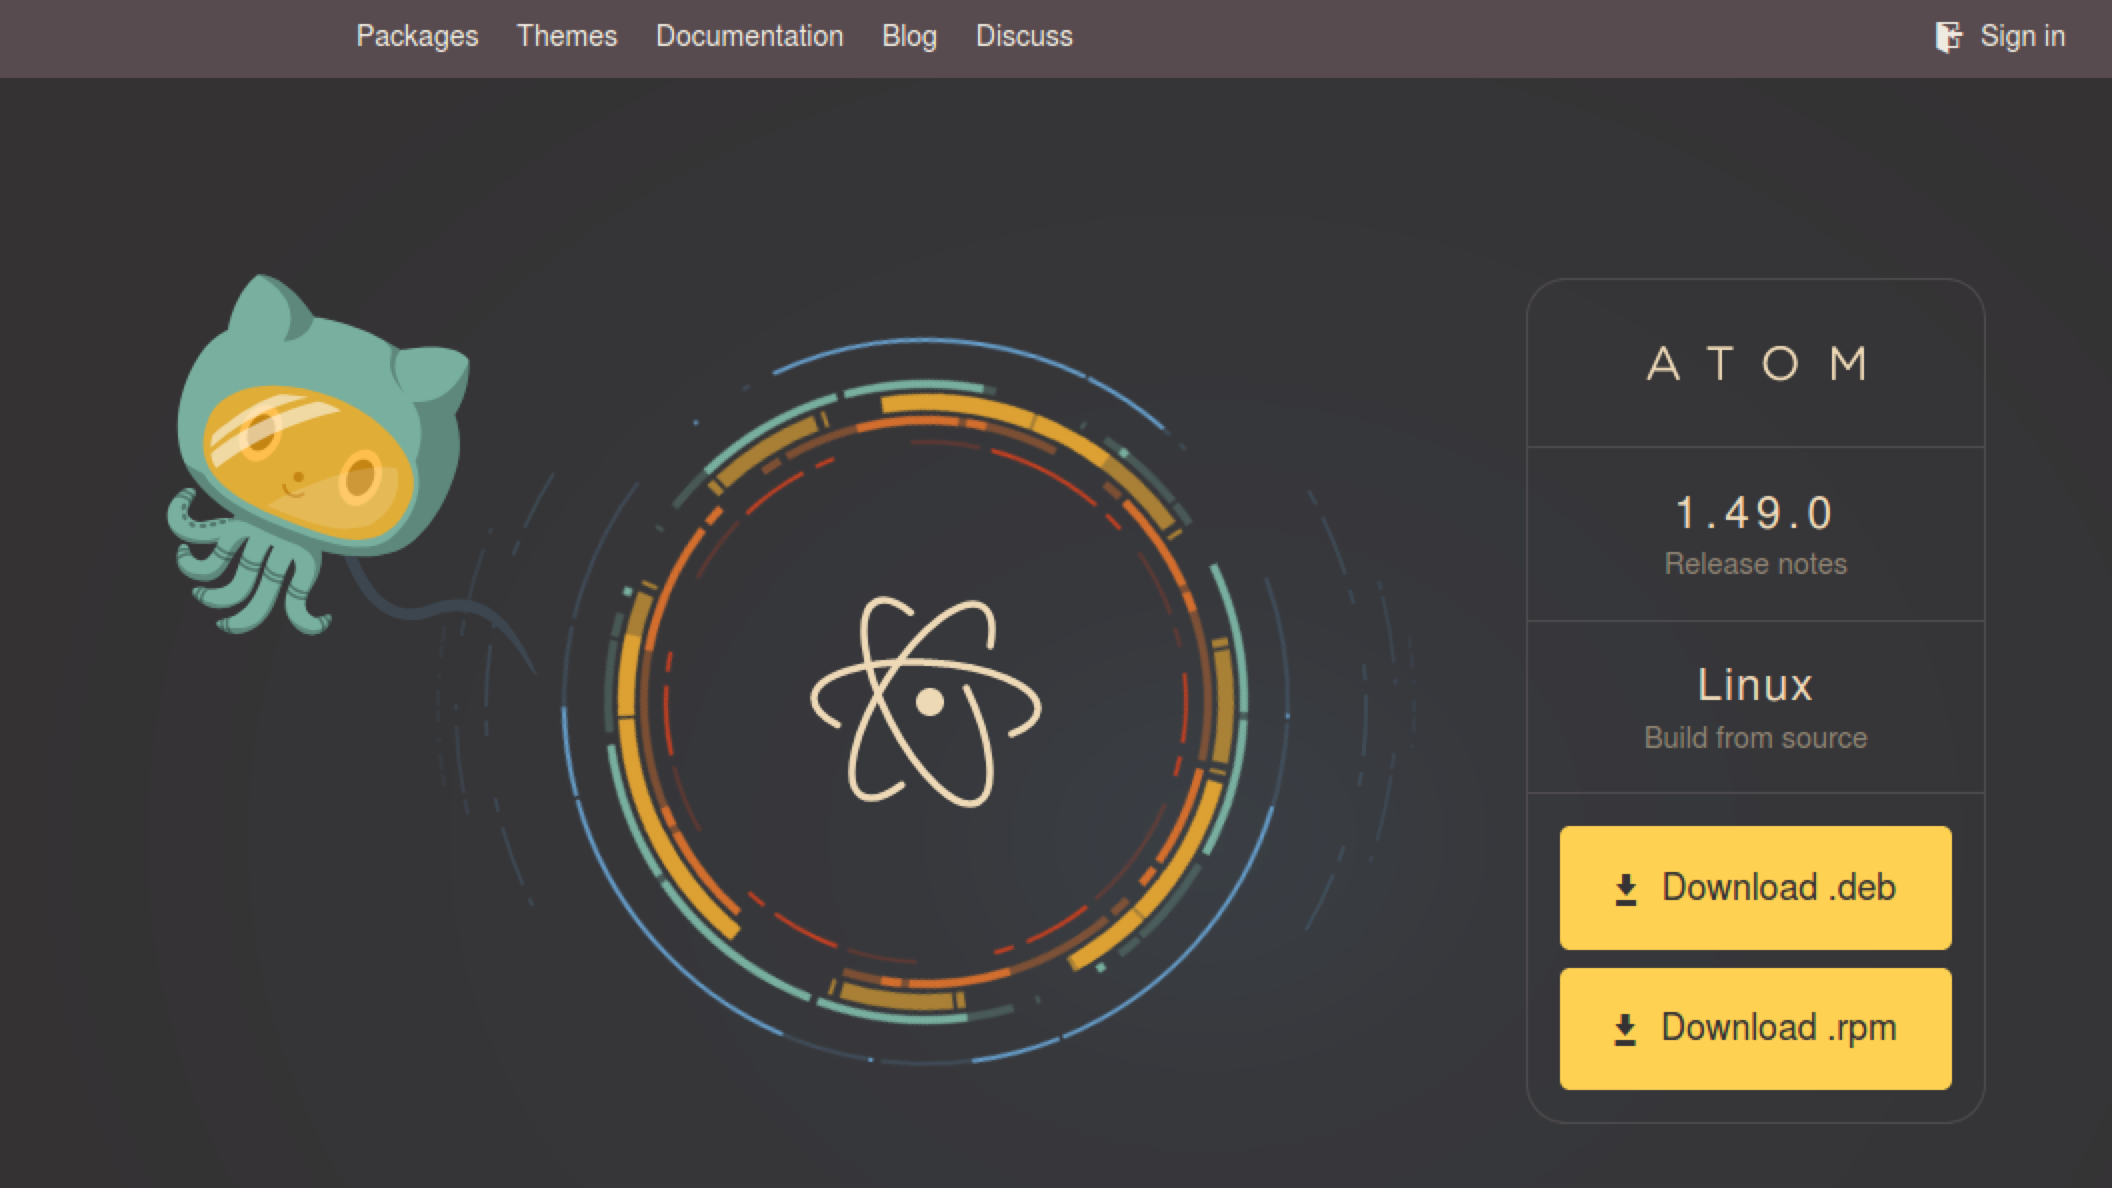
\includegraphics[width=1\columnwidth]{Pictures/atom_dl.png}}
\caption{Page d'accueil d'Atom}
\label{fig-page-atom}
\end{figure}
\begin{itemize}
\item Pour Mac et Windows, cliquez sur l’icône "télécharger" pour l’installer\footnote{il y a des risques d'incompatibilité des dernières versions d'Atom avec le package de gestion du LoPy (pymakr). Nous vous recommandons d'utiliser une version plus ancienne, comme la 1.44 disponible dans les archives d'Atom Release \url{https://github.com/atom/atom/releases/tag/v1.44.0}(\texttt{AtomSetup-x64.exe} pour Windows ou \texttt{atom-mac.zip} pour Mac OS).}.
\item Pour Linux, téléchargez le\texttt{.deb} et tapez \texttt{sudo dpkg -i atom-amd64.deb}\footnote{Il est possible qu'un message vous dise que git n'est pas installé. Dans ce cas, tapez \texttt{sudo apt-get install git} et suivez les instructions).}.
Lancez Atom en cliquant sur l’icône ou, sous Linux, en tapant atom dans un terminal.
\end{itemize}

     \vspace{1em}

Lancez Atom en cliquant sur l’icône ou, sous Linux, en tapant atom dans un terminal. L’écran d’accueil apparaît.

\subsection{Communiquez avec votre Pycom}

Pour communiquer avec le Pycom à travers Atom, vous devez installer le package pymakr.

Cliquez sur \textit{Install a Package} puis \textit{Open Installer}. Une autre fenêtre s’ouvre (cf. figure~\vref{fig-page-pakage}. Tapez \texttt{pymakr} dans le menu. Un package apparaît portant ce nom. Cliquez sur \textit{Install}. L’installation peut prendre plusieurs minutes. Vous avez le temps de prendre un café.

\begin{figure}[tbp]
\centerline{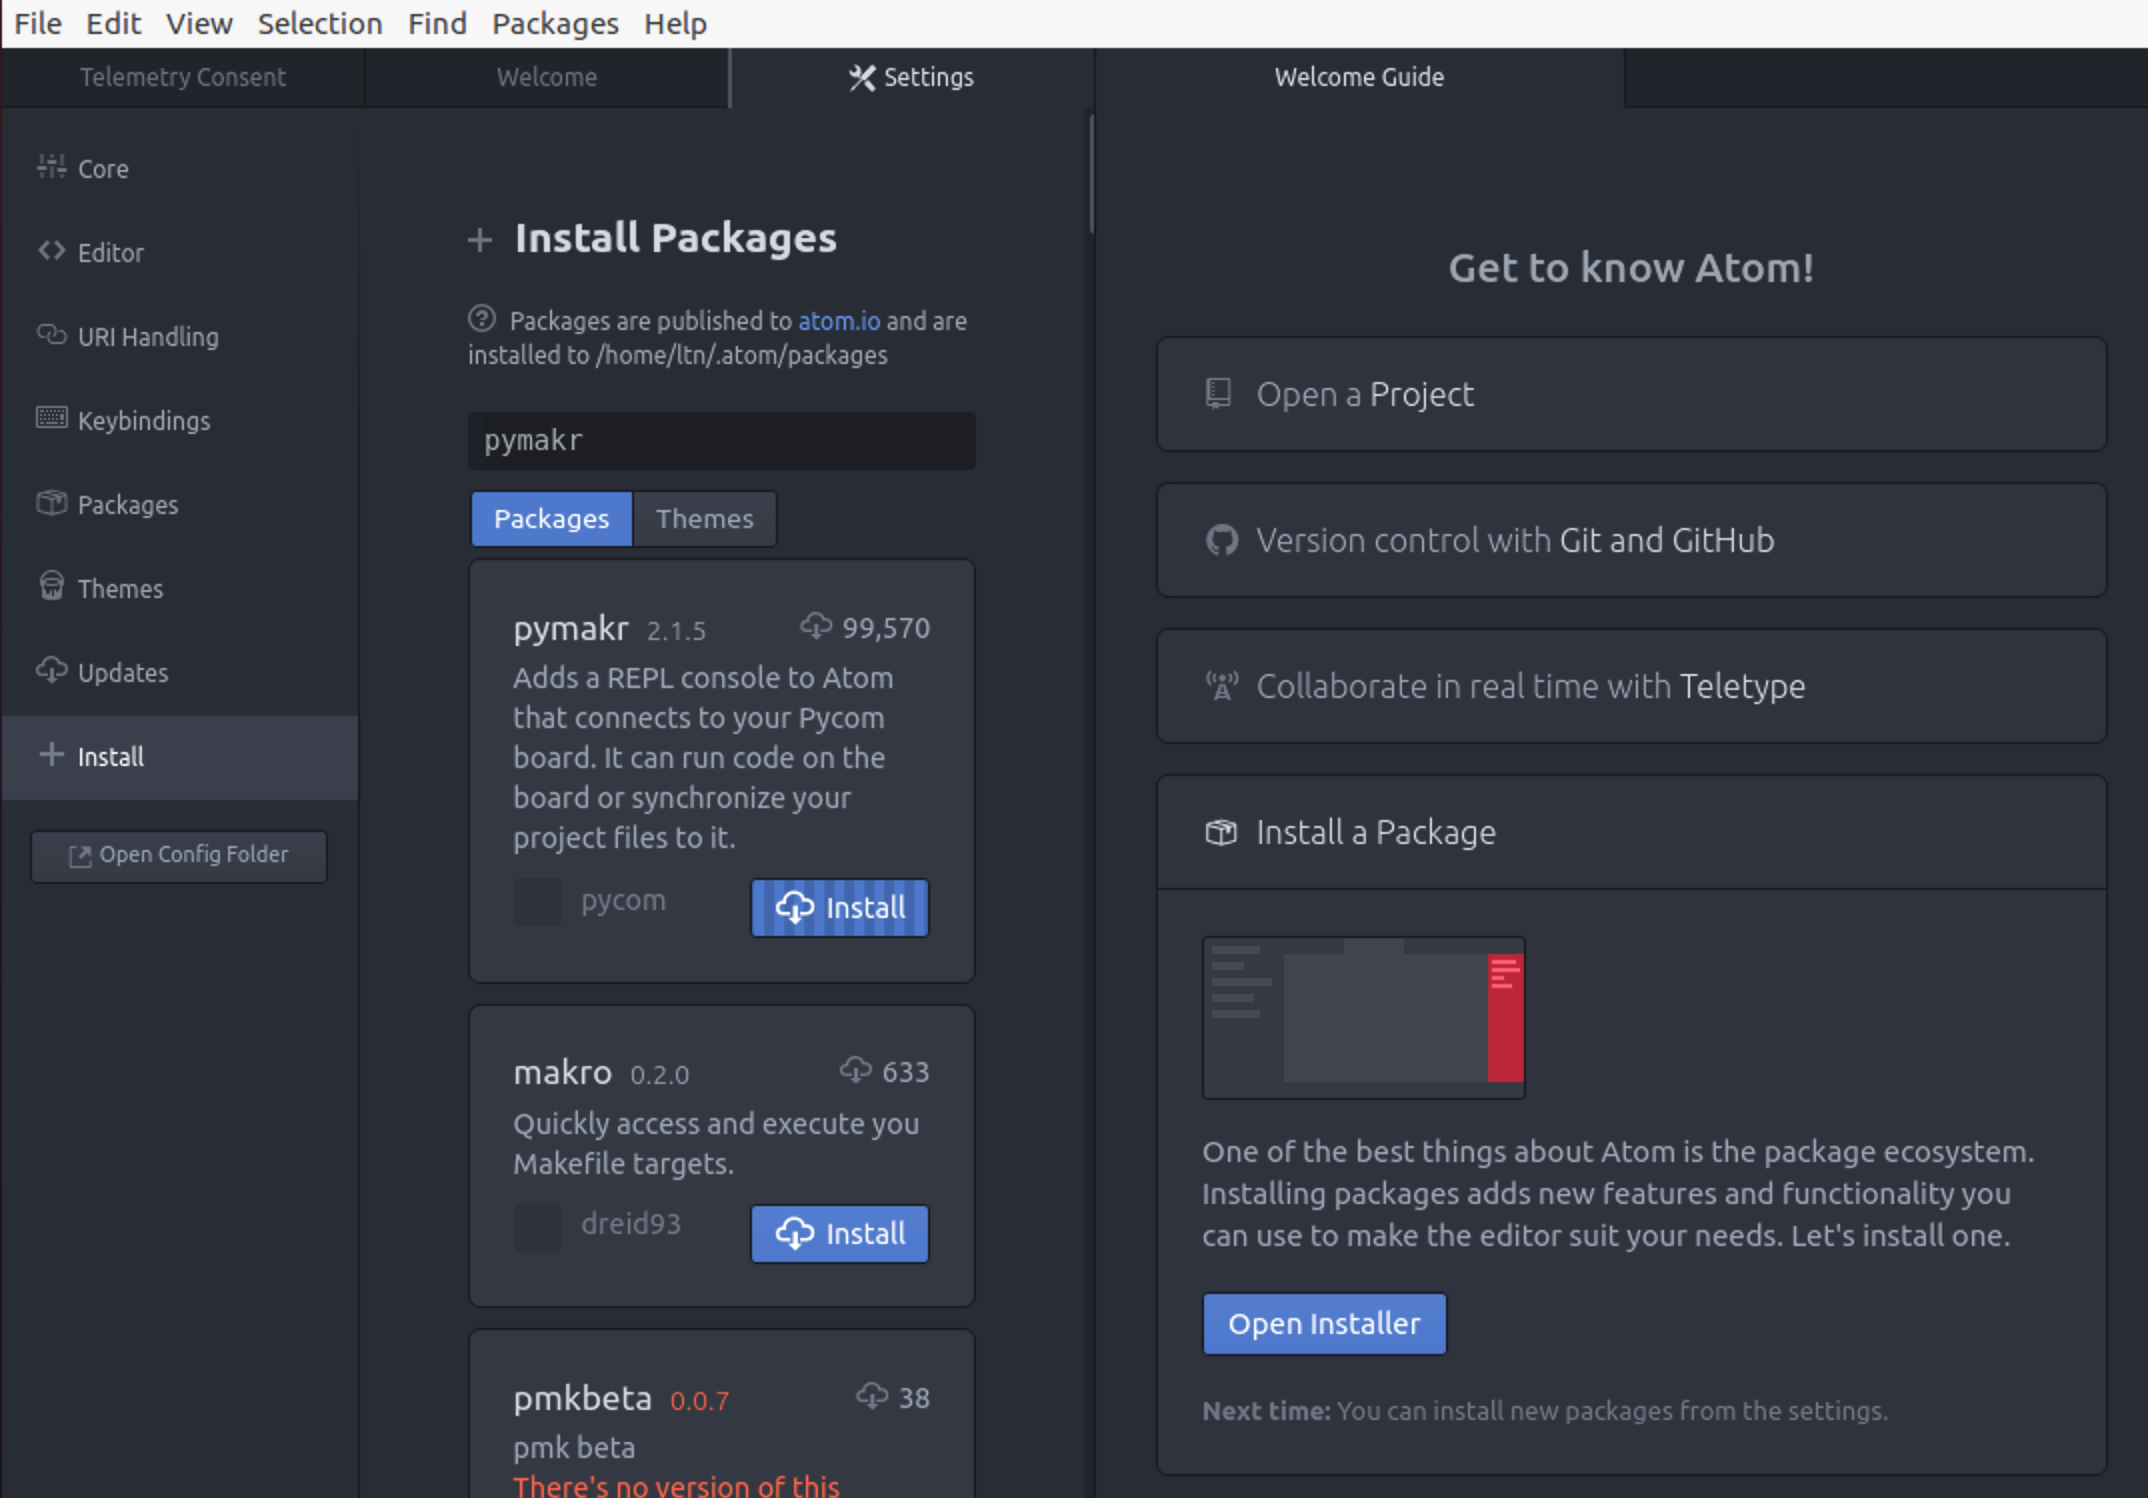
\includegraphics[width=1\columnwidth]{Pictures/atom_pymakr.png}}
\caption{Installation de Paquetages}
\label{fig-page-pakage}
\end{figure}

     \vspace{1em}

Une fois le café bu et l’installation terminée, une nouvelle fenêtre (terminal) s’ouvre en bas d’Atom.

     \vspace{1em}

Ce terminal (cf.figure~\vref{fig-page-pymakr}) vous permettra de dialoguer avec le LoPy. Branchez le LoPy à votre ordinateur. Vous devriez voir l’invite\texttt{ >{}>{}>{}} caractéristique d’un interpréteur Python\footnote{Sous Linux, vous devez être membre du groupe dialout pour pouvoir gérer la communication sur le port USB. Si vous ne voyez par l’invite, tapez sudo adduser login dialout en remplaçant login par le nom de votre compte Linux. Reconnectez-vous sous votre compte.}.

     \vspace{1em}

\begin{figure}[tbp]
\centerline{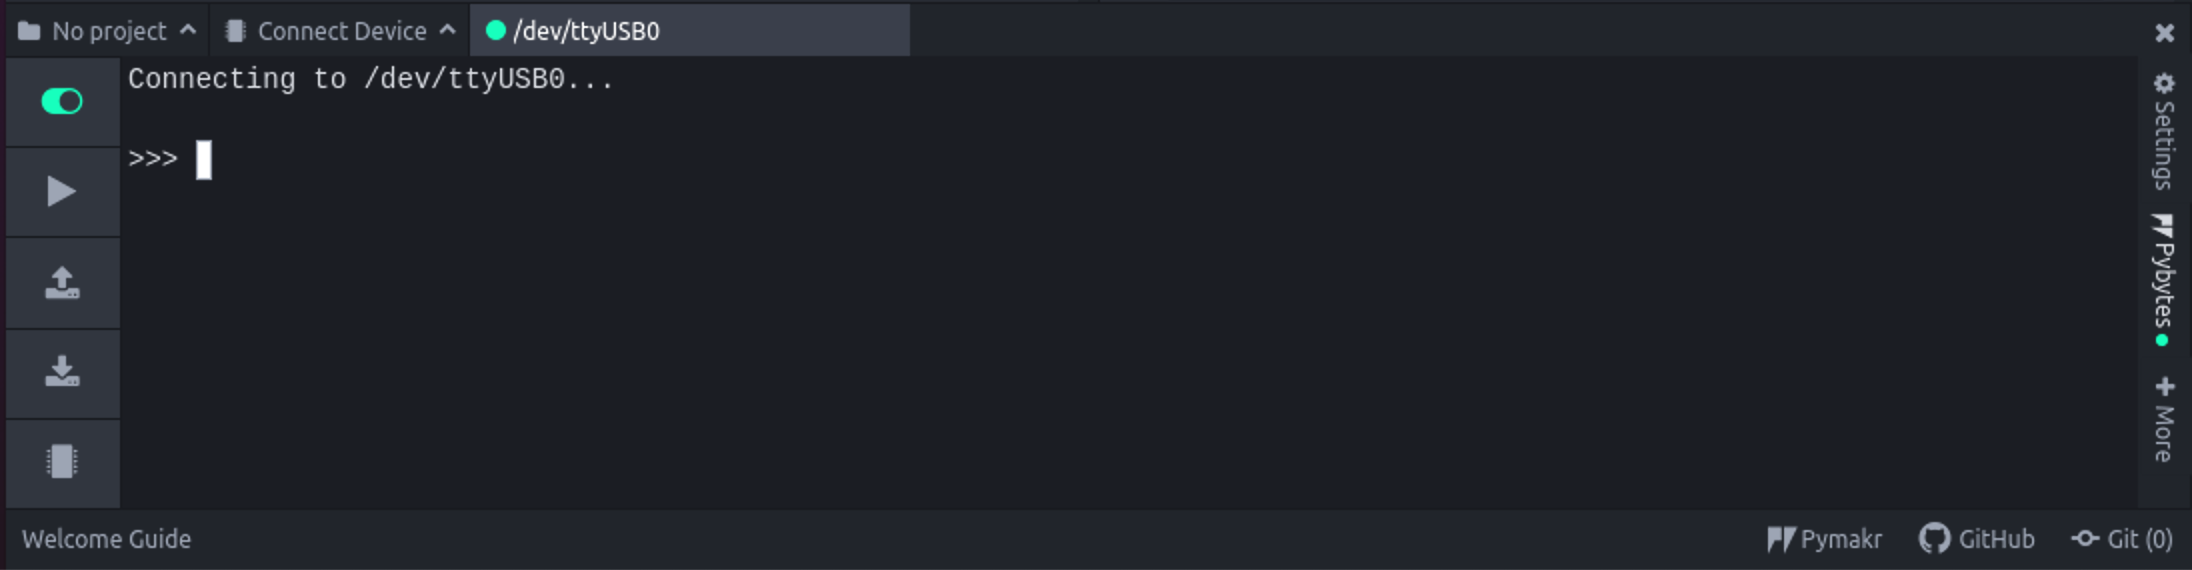
\includegraphics[width=1\columnwidth]{Pictures/atom_pymakr1.png}}
\caption{Fenêtre Pymakr}
\label{fig-page-pymakr}
\end{figure}

Toutes les commandes que vous allez taper dans cette fenêtre vont s’exécuter sur votre LoPy. Par exemple, si vous tapez\footnote{Les fenêtres sur fond gris montrent le code micropython et leur résultat.}~:

\begin{termc}[backgroundcolor=\color{gray!10}, language=json, basicstyle=\small, escapechar=@]
Connecting to /dev/ttyUSB0...
>>> @\textbf{1+1}@
2
>>>
\end{termc}

L’addition se fait sur le LoPy.

     \vspace{1em}

Sur le coté gauche de la fenêtre pymakr, plusieurs icônes sont présentes~:
\begin{itemize}
    \item l'interrupteur permet d'activer ou de désactiver le connexion avec le LoPy~;
    \item le triangle permet d'exécuter le programme affiché dans la fenêtre d'Atom sur le LoPy~;
    \item la flèche vers le haut, permet de recopier le répertoire actif dans la mémoire du LoPy. Cela sera utile pour installer de nouveaux modules sur le LoPy~;
    \item inversement le flèche vers le bas, permet de recopier la mémoire du LoPy sur l'ordinateur~;
    \item le processeur permet d'avoir des informations sur le loPy.
\end{itemize}

     \vspace{1em}

Sur la partie droite, l'onglet vertical \textit{Setting} permet de modifier les paramètres de connexion avec le LoPy.

\subsection{Installez votre environnement de travail} 

Comme pour dialoguer avec le pycom, nous n'allons pas utiliser la machine virtuelle, il reste à récupérer notre environnement de travail et les modules pour le Pycom.

Téléchargez tous les fichiers du dépôt github : https://github.com/ltn22/PLIDObis.git
Déposez-les dans un dossier de votre choix sur votre ordinateur.

Vous pouvez télécharger ce dépôt en une seule commande dans le répertoire de votre choix :

> git clone https://github.com/ltn22/PLIDObis.git
Allez ensuite dans le menu Files>Open Folder d’Atom, sélectionnez le répertoire pycom du dossier que vous venez de télécharger, et validez. Sur la partie gauche de l’écran, l’ensemble des fichiers composant ce répertoire doivent apparaître. Il y en a beaucoup, car ils vont nous servir tout au long de ce MOOC.

En cliquant dans la fenêtre pymakr sur le bouton Upload project to device, les fichiers de ce répertoire vont être copiés sur le Pycom. Par la suite, il faudra cliquer sur ce bouton pour copier les modifications que l’on pourrait faire sur le Pycom.